\section{Theoretische Grundlagen}
\label{sec:grundlagen}
%zugrundeliegende Theorien und Modelle
% Definitionen
% Stand der Technik, Normen und Standards, Wirtschaftliche Aspekte
% persönliche Positionierung

\subsection{Verdickungsmittel}

In der Farben- und Putzindustrie werden Verdickungsmittel als rheologische Additive bezeichnet. Sie erhöhen die Viskosität von Flüssigkeiten und ändern somit ihre rheologischen Eigenschaften, welche die Auftragungs-, Fließ- und Verlaufseigenschaften von Farben und Putzen bestimmen. Verdickungsmittel kommen jedoch auch in der Lebensmittelchemie oder Pharmazie zum Einsatz. Je nach dem welche Anforderungen an das Verdickermittel gestellt werden, unterscheiden sich diese in ihrer Zusammensetzung (siehe Abb. \ref{fig:verdicker_einteilung}). \cite{Brock.2009}

\begin{figure}[h!]
	\centering
	\begin{forest}
		forked edges,
		for tree={draw,align=center,edge={-latex}}
		[Verdickungsmittel, for children={fit=band}
			[Anorganisch]
			[Organisch, for children={fit=band}
				[Niedermolekular]
				[Synthetisch]
				[Natürlich, for children={fit=band}
					[Natürlich (abgewandelt)]
					]	
			]	
		]
	\end{forest}	
	\caption{Einteilung von Verdickungsmitteln nach Zusammensetzung \cite{Brock.2009}}
	\label{fig:verdicker_einteilung}
\end{figure}
\FloatBarrier

Je nach Verdickungsmittel können verschiedene Effekte wie Gelbildung, Solvatation, Ausbildung von Netzstrukturen, Coulomb-Kräfte, Quellung und Wasserstoff- Brückenbindungen, sowie deren gegenseitige Einflussnahme die Erhöhung der Zähflüssigkeit bewirken. \cite{Brock.2009} \\
Betrachtet man speziell die sogenannten assoziativen Verdickungsmittel lassen sich diese den Gruppen der abgewandelten, natürlichen Verdicker und den synthetischen Verdickern zuordnen.  Sie spezifizieren sich gegenüber anderen Verdickertypen darin, dass sie neben hydrophilen Gruppen auch hydrophobe End- und Seitengruppen enthalten, welche dem Verdickungsmittel einen Tensidcharakter verleihen. Deshalb bestehen assoziative Verdicker unteranderem aus hydrophob modifizierten Polymerstrukturen (siehe Abb. \ref{fig:assoziativ_einteilung}).

\begin{figure}[h!]
	\centering
	\begin{forest}
		forked edges,
		for tree={draw,align=center,edge={-latex}}
		[Assoziativverdicker
		[hydrophob \\ modifizierte \\ Polyacrylate]
		[hydrophob \\ modifizierte \\ Celluloseether]
		[hydrophob \\ modifizierte \\ Polyether]
		[hydrophob \\ modifizierte \\ Polyacrylamide]
		[assoziative \\ Polyurethan-Verdicker]
		]
	\end{forest}	
	\caption{Einteilung von Assoziativ-Verdickern nach chemischer Struktur \cite{Brock.2009}}
	\label{fig:assoziativ_einteilung}
\end{figure}
\FloatBarrier
Diese strukturelle Eigenschaft der Assoziativ-Verdicker macht die Bildung von Micellen möglich und es treten neben der Quellung in der Wasserphase sogenannte "`Micellbrücken"' zwischen Latex-Teilchen der Bindemitteldisperion auf, welche eine zusätzlich Viskositätserhöhung bewirken. \cite{Brock.2009} \\
In Abbildung \ref{fig:struktur_puverdicker} ist eine schematische Struktur eines solchen assoziativen Polyurethan-Verdickers aufgeführt. Diese beispielhafte Struktur zeigt hydrophile, höher molekulare Polyethersegmente, welche über Urethan-Gruppen verbunden sind und durch hydrophobe Molekülgruppen verknüpft werden. \cite{Brock.2009}

\begin{figure}[h!]
	\centering
	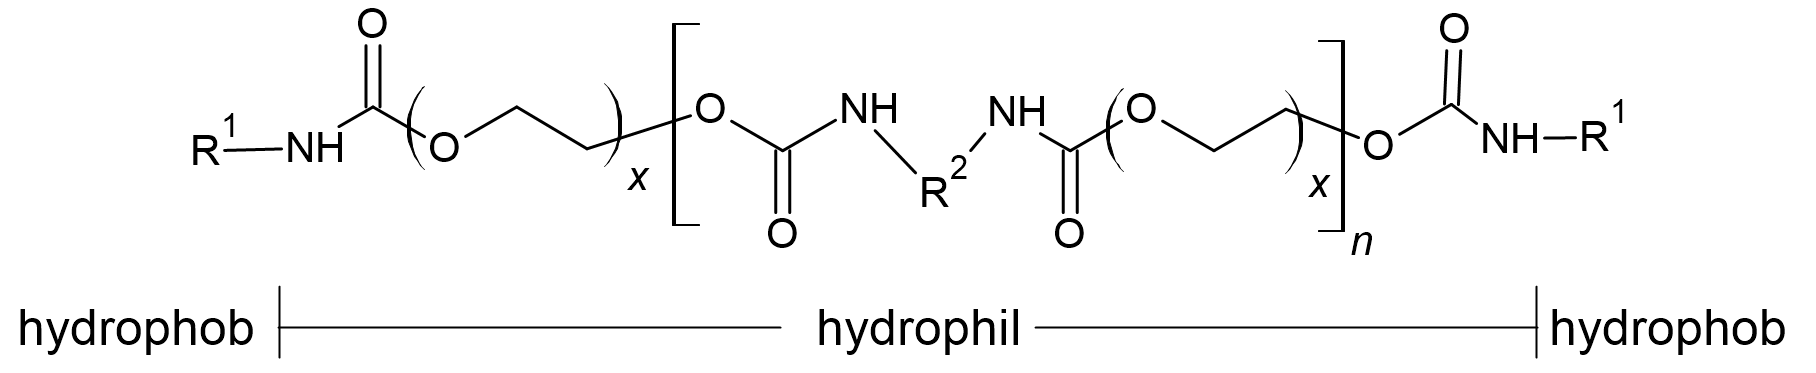
\includegraphics[width=0.75\textwidth]{img/verdicker_struktur}
	\caption{schematische Struktur eines assoziativen Polyurethan-Verdickers, \linebreak erstellt nach \cite{Brock.2009}}
	\label{fig:struktur_puverdicker}
\end{figure}
\FloatBarrier

Durch diesen Mix der hydrophoben und hydrophilen Strukturen wird der Tensidcharakter des Verdickungsmittels bestimmt und es ergeben sich Netzstrukturen mit assoziierten "`Micellbrücken"', wie in Abbildung \ref{fig: verdicker_anwendung} dargestellt. Zusätzlich ist zu erkennen, dass auch Wechselwirkungen mit bereits vorhandenen Tensidmolekülen in der Dispersion auftreten können und die Struktur somit weiter stabilisieren. \cite{Mezger.2016}

\begin{figure}[h!]
	\centering
	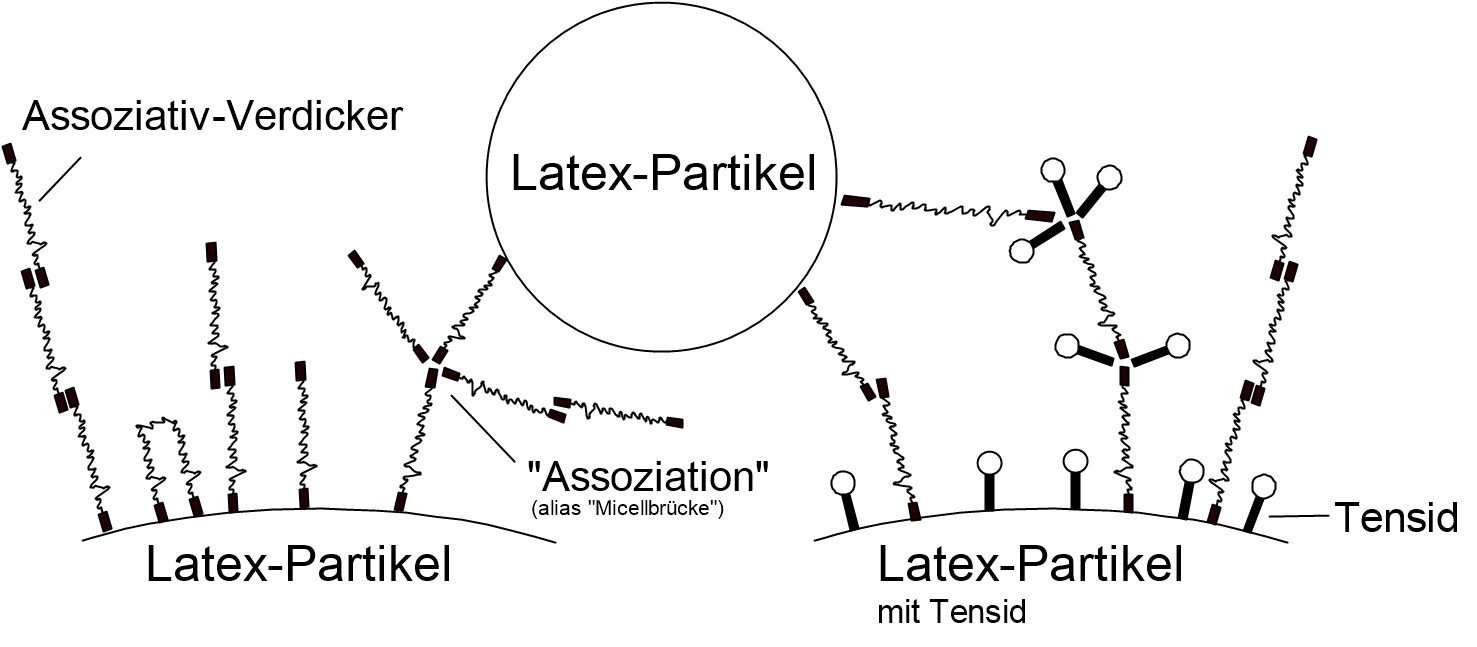
\includegraphics[width=0.75\textwidth]{img/verdicker_anwendung}
	\caption{Netzstruktur durch Verdickermittel in Latex-Dispersion (mit und ohne Tensid), \linebreak erstellt nach \cite{Mezger.2016}}
	\label{fig: verdicker_anwendung}
\end{figure}
\FloatBarrier

Aufgrund dieser ausgeprägten Netzstrukturen innerhalb des Verdickungsmittels ist es jedoch auch möglich, dass das Verdickungsmittel selbst eine hohe Viskosität aufweist. Dieser Punkt kann erheblichen Einfluss auf die großtechnische Verarbeitbarkeit des Additives haben und wird im weiteren Verlauf dieser Arbeit näher betrachtet. 

\subsection{Charakterisierung des Dosierstroms}

\subsubsection*{Rheologie von Fluiden}
Die Wissenschaft der Rheologie beschäftigt sich unter anderem mit dem Fließ- und Deformationsverhalten von Flüssigkeiten und teilt diese zunächst in \textsc{Newtonsche} und \textsc{Nichtnewtonsche} Fluide ein. Grundlage dieser Einteilung sind Untersuchungen von \textsc{Isaac Newton}, welcher sich bei konstanter Temperatur mit der Schergeschwindigkeit $D$ in Abhängigkeit von der Schubspannung $\tau$ beschäftigte. 
Das Ergebnis dieser Arbeit ist das \textsc{Newtonsche Fließgesetz} unter \linebreak Gleichung \eqref{eq: newton}, welche den Fließwiderstand $\eta$ einer Flüssigkeit bei gegebener Temperatur als Stoffkonstante benennt. Dieser Fließwiderstand $\eta$ ist heute unter der Bezeichnung der dynamischen Viskosität bekannt.

\begin{equation}
	\label{eq: newton}
	\tau = \eta * D
\end{equation}
\begin{parameter}
	D 			& Schergeschwindigkeit\\
	\tau 		& Schubspannung\\
	\eta 		& Dynamische Viskosität\\
\end{parameter}

Demnach gelten alle Fluide, welche diese Linearität zwischen Schergeschwindigkeit und Schubspannung ohne Fließgrenze aufweisen als \textsc{Newtonsche} Fluide und diejenigen, die ein nicht-lineares Verhalten und/oder ein Verhalten mit Fließgrenze aufweisen als \textsc{Nichtnewtonsche} Fluide. Veranschaulicht wird dies in Abbildung\,\ref{fig: arten_fluide} mit einer Auswahl an verschiedenen Rheologieprofilen.

\begin{figure}[h!]
	\begin{minipage}[b]{0.475\textwidth}
		\includegraphics[width=\textwidth]{img/fluidarten}
		\caption{Fließkurven für verschiedene \linebreak Fluide, erstellt nach \cite{Holze.2010}}
		\label{fig: arten_fluide}
	\end{minipage}
	\hspace*{0.05\textwidth}
	\begin{minipage}[b]{0.475\textwidth}
		\includegraphics[width=\textwidth]{img/fluidarten2}
		\caption{Viskositätskurven für verschiedene Fluide, erstellt nach \cite{MunzingChemieGmbH.2018}}
		\label{fig: arten_fluide2}
	\end{minipage}
\end{figure}
\FloatBarrier

\subsubsection*{Bestimmung der dynamischen Viskosität nach DIN EN ISO 2555}
Eine Möglichkeit die dynamische Viskosität einer Dispersion zu bestimmen, ist die Messung mit einem Rotationsviskosimeter nach DIN EN ISO 2555. Da in dieser Norm hauptsächlich ein Rotationsviskosimeter mit Einzelzylinder beschrieben ist, wird an dieser Stelle auf die DIN ISO 3219 verwiesen. In dieser Norm werden zusätzlich Rotationsviskosimeter mit koaxialem Zylinder und Kegel-Platte-Viskosimeter näher beschrieben. \cite{DINDeutschesInstitutfurNormunge.V..Februar2013, DINDeutschesInstitutfurNormunge.V..September2018} \\
Allgemein beschreiben Rotationsviskosimeter einen Viskosimetertypen, bei dem die zu messende Flüssigkeit zwischen spezifisch geformten Körpern gebracht wird, von denen einer rotiert. Dabei tritt eine Scherung der Flüssigkeit auf und das aufgewendete Drehmoment am Viskosimeter wird gemessen. Neben Rotationsviskosimetern sind auch weitere Viskosimetertypen wie Kappilarviskoskosimeter und Fallkörperviskosimeter bekannt. Diese unterscheiden sich gegenüber dem Rotationsviskosimeter beispielsweise darin, dass sie im Regelfall die Viskosität von \textsc{Nichtnewtonschen} Fluiden nicht ausreichend untersucht werden kann. \cite{ROMPPRedaktion.2008}

Das bei \textsc{Alberdingk Boley Leuna GmbH} verwendete Verfahren zur Viskositätsbestimmung ist angelehnt an die DIN EN ISO 2555 unter Nutzung eines digitalen \textsc{Brookfield}-Rotationsviskosimeters, benannt nach dem Hersteller \textsc{AMETEK$^\text{\textregistered}$\,Brookfield}. Diese Viskosimeter haben den Vorteil preisgünstig zu sein und erlauben ein Messen der Viskosität direkt im Probengefäß. Da jedoch durch das direkte Eintauchen in ein theoretisch beliebiges Probengefäß nur eingeschränkte Übertragbarkeiten und Reproduzierbarkeiten möglich sind, können diese Geräte hauptsächlich für Vergleichsmessungen genutzt werden.  Der Hersteller gibt hierfür an ein \SI{600}{\milli \liter} Becherglas als Probengefäß zu nutzen, jedoch wird in der DIN\,EN\,ISO\,2555 darauf hingewiesen, dass die Becherglasgröße freigewählt werden darf. Für den Vergleich von Messungen rät die Norm dennoch jeweils die gleiche Größe des Becherglases zu nutzen. \cite{ROMPPRedaktion.2008, brookfield_31.01.2022, DINDeutschesInstitutfurNormunge.V..September2018}

\begin{wrapfigure}{R}{0.33\textwidth}
	\centering
	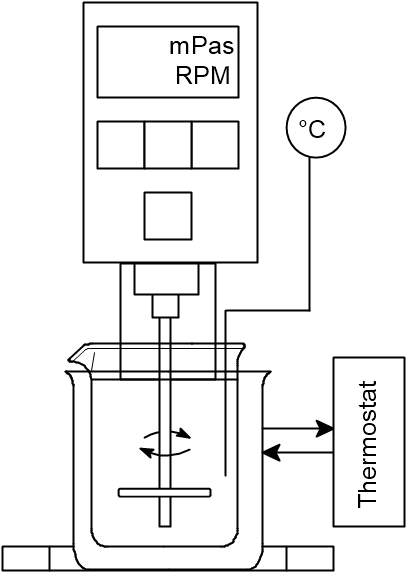
\includegraphics[width=0.25\textwidth]{img/viskosimeter}
	\caption{Viskositätsmessung mit digitalem \textsc{Brookfield}-\linebreak Rotationsviskosimeter}
	\label{fig: viskosimeter}
\end{wrapfigure}
\FloatBarrier
%Ende

Die Messung mittels digitalem \textsc{Brookfield}- \linebreak Viskosimeters ist vergleichsweise einfach. Benötigt werden hierfür das Viskosimeter in einer Halterung, ein Becherglas, ein Temperaturmessgerät und eine herstellerspezifische Spindel. Soll die Viskosität bei bestimmten Temperaturen, abweichend der Labortemperatur bestimmt werden, ist zusätzlich ein thermostatisches Flüssigkeitsbad nötig (vgl. Abb. \ref{fig: viskosimeter}). Die Messung lässt sich nach dem Aufbau über das Bedienfeld starten in dem Spindel und Drehzahl eingegeben werden. \linebreak Sobald die Messung startet beginnt sich die Spindel zu drehen.\\
Das Messprinzip eines solchen \textsc{Brookfield}- \linebreak Viskosimeters basiert auf der Messung der Winkelabweichung, auch Torsion genannt, zwischen der im Viskosimeter verbauten Welle und einer zweiten darunter angeordneten Spindel-Welle mit fest definierten geometrischen Körper. Beide Wellen drehen sich dabei mit der selben Drehzahl  und sind über eine Federeinheit verbunden. Bei Digital-Viskosimetern wird der Messwert der sich dann durch die Winkelabweichung ergibt direkt über ein Display angezeigt.\\
Entscheidend für die Messung der Viskosität ist bei dieser Messmethode die Auswahl des bereits erwähnten Becherglases, sowie der Spindel und der Drehzahl. Spindel und Drehzahl werden dabei unter Einbezug des Viskositätbereiches der Probe nach der gewünschten Präzision und dem Geschwindigkeitgefälle ausgewählt. \cite{DINDeutschesInstitutfurNormunge.V..September2018} 
Durch Tabellen des Herstellers, welche sowohl Spindel als auch Viskositätsbereich in Abhängigkeit von Drehzahl und Gerätekonstanten berechnen lassen, werden diese Entscheidungen vereinfacht. \cite{brookfield_31.01.2022} 


\subsubsection*{Bestimmung der Strömungsform}
Um den Dosierstrom des Verdickermittels entsprechend seiner Strömungseigenschaften charakterisieren zu können, wird zunächst mit der sogenannten \textsc{Reynoldszahl} die Strömungsform bestimmt. Sie ist eine dimensionslose Kennzahl und beschreibt das Verhältnis zwischen Tragheitskräften zu Reibungskräften in strömenden Flüssigkeiten und ist für durchströmte Rohrleitungen unter Gleichung \eqref{eq: reynolds} definiert. \cite{Foth.2014}

\begin{equation}
	\label{eq: reynolds}
	Re = \frac{d_H*\rho*\overline{u}}{\eta}
\end{equation}
\begin{parameter}
	Re 			& 	\textsc{Reynoldszahl} \\
	\eta 		& dynamische Viskosität des Fluids\\
	\rho 		& Dichte des Fluids\\
	d_H			&	hydraulischer Rohrdurchmesser\\
	\overline{u} & mittlere Strömungsgeschwindigkeit\\
\end{parameter}

Anhand der Reynoldszahl lässt sich nun mithilfe der Tabelle \ref{tab:stromung_reynolds}, die jeweilige Strömungsform zuordnen. Diese Zuordnung ist wichtig, da sich je nach Strömungsform unterschiedliche Einflussgrößen auf den Druckverlust ergeben. Beispielsweise hat für eine laminare Strömung die Wandrauigkeit der Leitung keinen Einfluss mehr, wohin gegen sie in turbulenten Strömungen maßgebliche Druckverluste hervorrufen kann. In laminaren Strömungen überwiegt hierbei der glättende Einfluss der Viskosität gegenüber den Rohrunebenheiten, während in turbulenten Strömungen weitere Wirbel erzeugt werden. \cite{Bschorer.2018}

% Table generated by Excel2LaTeX from sheet 'Daten'
\begin{table}[h!]
	\renewcommand*{\arraystretch}{1.2}
	\centering
	\rowcolors{2}{white}{gray!25}
	\caption{Strömungsformen und ihre Reynoldszahlen \cite{Foth.2014}}
	\label{tab:stromung_reynolds}
	%\resizebox{10.5cm}{!}{
		\begin{tabulary}{1.0\textwidth}{C|CCC}
			\hline
			\textbf{Strömungsform} & \textbf{Laminar} & \textbf{instabiler Bereich} & \textbf{Turbulent}\\
			\hline
			\textbf{Reynoldszahl} &	$< 2300$ & $2300$ bis $4000$& $>4000$\\
			\hline			
	\end{tabulary}
%}
\end{table}%
\FloatBarrier

\subsubsection*{Bestimmung des Druckverlustes}
Nach der Bestimmung der Reynoldszahl lässt sich nun mit Hilfe des \linebreak \textsc{Nikuradse-Colebrook-Moody}-Diagramms, nachfolgend \textsc{Moody}-Diagramm genannt, der Rohrreibungsbeiwert $\lambda$ bestimmen (siehe Abb. \ref{fig:moody}). Dieser Wert wiederum kann in Gleichung \eqref{eq:druckverlustbeiwert} eingesetzt werden um den Druckverlustbeiwert $\zeta_R$ für gerade Rohrleitungen zu bestimmen und lässt auf Basis der erweiterten \textsc{Bernoulli}-Gleichung \eqref{eq:druckverlust_zeta} den durch Reibung verursachten Druckverlust $\Delta p$ berechnen. \cite{Bschorer.2018}

\begin{equation}
	\label{eq:druckverlustbeiwert}
	\zeta_R = \lambda * \frac{L}{d}
\end{equation}
\begin{equation}
	\label{eq:druckverlust_zeta}
	\Delta p = \frac{1}{2}*\zeta_R*\rho*\overline{u}^2
\end{equation}
\begin{parameter}
	\zeta_R		& Druckverlustbeiwert für gerade Rohrstrecken\\
	L 			& Rohrleitungslänge\\
	d			& Rohrdurchmesser\\
	\Delta p	& Druckverlust \\
	\rho 			& Dichte des Fluids\\
	\overline{u} 	& mittlere Strömungsgeschwindigkeit\\
\end{parameter}


\begin{figure}[h!]
	\centering
	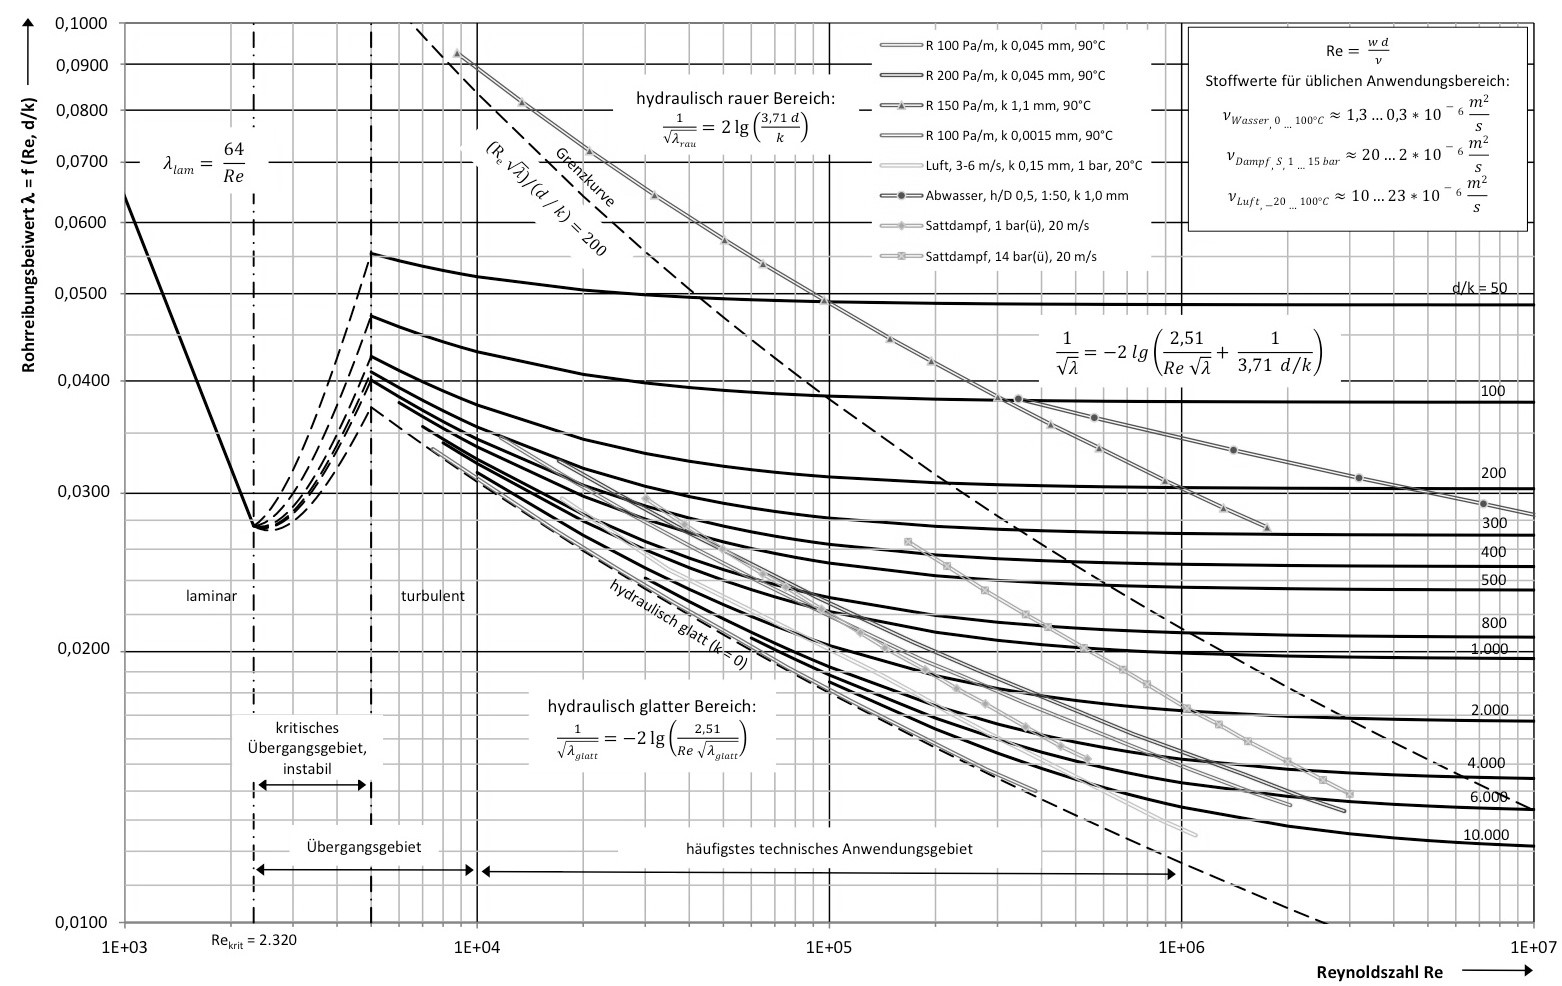
\includegraphics[width=1.0\textwidth]{img/R_Rohrreibungsbeiwert.jpg}
	\caption{\textsc{Nikuradse-Colebrook-Moody}-Diagramm \cite[\ccbysa]{Msimca.2017}}
	\label{fig:moody}
\end{figure}
\FloatBarrier
%Ende


\subsubsection*{Gesetz von  \textsc{Hagen}-\textsc{Poiseuille}}
Liegt für eine nicht-kompressible Flüssigkeit eine laminare Strömung vor, so ist es möglich die zuvor beschriebene Vorgehensweise zu vereinfachen und den auftretenden Druckverlust in einer geraden Rohrleitung direkt mit dem Gesetz von \textsc{Hagen}-\textsc{Poiseuille} zu bestimmen.  Der Druckverlust wird hierbei in Abhängigkeit vom Volumenstrom, der Rohrleitungslänge, des Rohrdurchmessers und der Viskosität berechnet. Die Definition des Gesetzes, aufgelöst nach dem Druckverlust, findet sich unter Gleichung \eqref{eq:hagen}. \cite{Foth.2005}

\begin{equation}
	\label{eq:hagen}
	\Delta p  = \frac{8*\eta*L*\dot{V}}{r^4*\pi}
\end{equation}
\begin{parameter}
	\Delta p	& Druckverlust \\
	\eta 		& dynamische Viskosität des Fluids\\
	\dot{V}		& Volumenstrom des Fluids\\
	r			& innerer Radius der Rohrleitung\\
	L 			& Rohrleitungslänge\\
\end{parameter}

Da das Gesetz von \textsc{Hagen}-\textsc{Poiseuille} bereits im \textsc{Moody}-Diagramm enthalten ist, können beide Vorgehensweisen genutzt werden um die jeweils andere Rechnung zu überprüfen. Sollen Rohrleitungseinbauten wie Armaturen, Ventile oder Bogenstücke einberechnet werden, vereinfacht jedoch aufgrund von tabellierten Druckverlustbeiwerten möglicher Einbauten die erweiterte \textsc{Bernoulli}-Gleichung die Berechnung des gesamten reibungsbedingten Druckverlustes.

\subsection{Gebindeformen für Flüssigkeiten}
Um ein Edukt neu in die Produktion einzubinden sind, nicht nur die chemisch-physikalischen Eigenschaften relevant. Auch der Aspekt der Gebindeform ist maßgeblich für die Einfügung des Eduktes in den Produktionsablauf. Für flüssige Edukte sind im Tagesgeschäft der \textsc{Alberdingk Boley Leuna GmbH} hauptsächlich IBCs (Intermediate Bulk Container) und zum Teil Kunststoff-Deckelfässer im Einsatz. Es sei jedoch erwähnt, dass auch weitere Gebinde auf dem Verpackungsmarkt verfügbar sind, wie beispielsweise Kanister, Hobbocks oder Metallfässer.\\
Den IBC als kubisches Gebinde gibt ca. seit den 1960er Jahren  und hat sich über eine Richtlinie des VDI aus den frühen 70er-Jahren zu einem Standard der großen Einzelverpackungen entwickelt. Zuvor waren zum Großteil \SI{200}{\liter}-Fässer im Einsatz, welche sich neben der geometrischen Form auch maßgeblich im Handling unterscheiden. \cite{neueverpackung.01.02.2022}
So lassen sich Fässer in dieser Größenordnung beispielsweise im Regelfall nur als 4er-Packung sicher transportiert werden und benötigen hierfür zusätzliche Paletten, sowie Schrumpffolie um die Behälter zu fixieren. Ein IBC hingegen kann direkt als Gebinde mit einem Hubwagen oder Gabelstapler transportiert werden. Weitere Punkte im Vergleich zwischen IBC und Fass finden sich unter Tabelle \ref{tab:ibc_fass}.

\missingfigure{Tabelle mit Vergleich zwischen IBC und Fass fehlt}
%Anschlüsse ergänzen IBC und FASS

\todo[inline]{Fazit aus Tabelle}

\subsection{Dosierpumpen}

\subsubsection{oszillierende Verdrängerpumpen}

\subsubsection{rotierende Verdrängerpumpen}

\subsection{Bestimmung des Dosierstroms}
\subsubsection*{Radarfüllstandsmessung}
\subsubsection*{Coriolis-Massendurchflussmesser}
\subsubsection*{Volumetrischer Verdränger}
\subsubsection*{Waage mit Wägezellen}
\subsubsection*{Durchflusskurve der Pumpe}




%\subsection{Normen und Standards}
%
%
%\subsection{Densimeter}
%
%Norm für Viskositätsbestimmung
%
%https://www.din.de/de/neuer-inhalt/wdc-beuth:din21:306904236
%https://www.din.de/de/wdc-beuth:din21:512291
%https://www.din.de/de/neuer-inhalt/wdc-beuth:din21:329765890
%
%\subsection{Wirtschaftliche Aspekte und Entwicklungsperspektiven}